\documentclass[border=2pt]{standalone}
\usepackage[T1]{fontenc}
\usepackage{tikz}
\usepackage{amsmath,amssymb}
\usepackage{graphicx}
\usetikzlibrary{positioning, arrows.meta, fit, backgrounds, calc, decorations.pathreplacing}

% === Color palette ===
\definecolor{cBlue}{HTML}{3B7DD8}
\definecolor{cGreen}{HTML}{27AE60}
\definecolor{cPurple}{HTML}{8E44AD}
\definecolor{cGray}{HTML}{5D6D7E}

\begin{document}
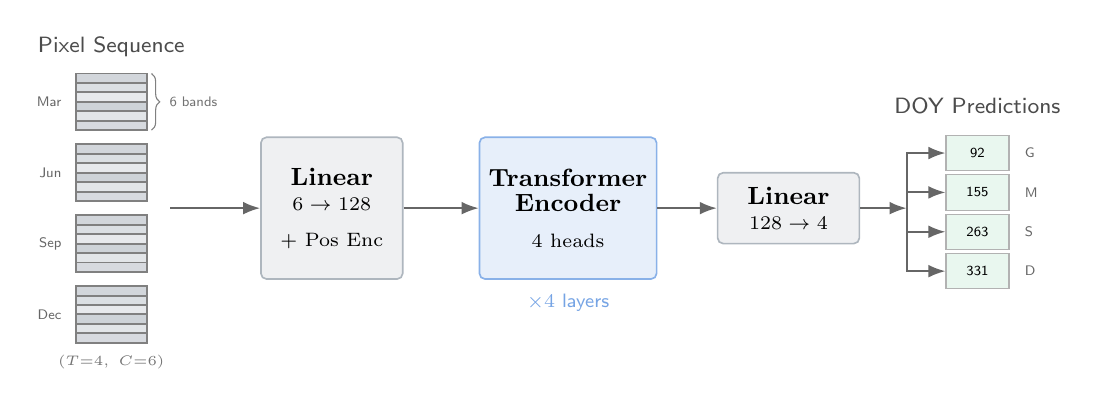
\begin{tikzpicture}[
    >=Latex,
    block/.style={
        draw, rounded corners=2pt, minimum height=0.9cm,
        align=center, font=\small, line width=0.6pt
    },
    pb/.style={block, fill=cBlue!12, draw=cBlue!60},
    gb/.style={block, fill=cGray!10, draw=cGray!50},
    fb/.style={block, fill=cPurple!12, draw=cPurple!60},
    arr/.style={->, line width=0.7pt, draw=black!60},
    garr/.style={->, line width=0.7pt, draw=cGreen!70},
    shp/.style={font=\tiny\sffamily, text=black!55},
    fmap/.style={draw, line width=0.5pt, rounded corners=0.5pt},
]

% =============================================
% INPUT: pixel temporal sequence (4 layered-band squares)
% =============================================

% Each square: 6 horizontal gray stripes representing 6 spectral bands
% Parameters
\def\sqW{0.9}       % square width in cm
\def\bandH{0.12}    % height of each band stripe
\def\sqX{0}         % x center of squares

% --- Helper: draw one timestep square at (#1 = y-center), label #2 ---
% 6 bands stacked, alternating gray shades, bold internal borders
\newcommand{\inputsquare}[2]{%
    \pgfmathsetmacro{\ybot}{#1 - 3*\bandH}%
    \foreach \b/\shade in {0/25, 1/18, 2/30, 3/15, 4/22, 5/28} {
        \pgfmathsetmacro{\by}{\ybot + \b*\bandH}%
        \fill[cGray!\shade] (\sqX - \sqW/2, \by) rectangle (\sqX + \sqW/2, \by + \bandH);
        % bold border for each band cell
        \draw[black!50, line width=0.7pt] (\sqX - \sqW/2, \by) rectangle (\sqX + \sqW/2, \by + \bandH);
    }
    % month label to the left
    \node[font=\tiny\sffamily, text=black!60, anchor=east] at (\sqX - \sqW/2 - 0.06, #1) {#2};
}

% Draw the 4 timestep squares with clear white-space gaps
% Total height per square = 6 * 0.12 = 0.72cm; gap ~0.22cm between squares
\inputsquare{0.15}{Mar}
\inputsquare{-0.75}{Jun}
\inputsquare{-1.65}{Sep}
\inputsquare{-2.55}{Dec}

% "6 bands" label + brace over the top square
\draw[decorate, decoration={brace, amplitude=3pt, mirror}, line width=0.4pt, draw=black!50]
    (\sqX + \sqW/2 + 0.06, 0.15 - 3*\bandH) -- (\sqX + \sqW/2 + 0.06, 0.15 + 3*\bandH)
    node[midway, right=3pt, font=\tiny\sffamily, text=black!55] {6 bands};

\node[font=\footnotesize\sffamily, text=black!70] at (\sqX, 0.85) {Pixel Sequence};
\node[shp] at (\sqX, -3.15) {$(T{=}4,\; C{=}6)$};

% =============================================
% LINEAR PROJECTION + POSITIONAL ENCODING
% =============================================

\node[gb, minimum width=1.8cm, minimum height=1.8cm] (proj) at (2.8, -1.2) {
    \textbf{Linear}\\[-2pt]
    {\scriptsize $6 \to 128$}\\[2pt]
    {\scriptsize + Pos Enc}
};

\draw[arr] (0.75, -1.2) -- (proj.west);

% =============================================
% MULTI-HEAD ATTENTION (Transformer Encoder)
% =============================================

\node[pb, minimum width=2.0cm, minimum height=1.8cm] (mha) at (5.8, -1.2) {
    \textbf{Transformer}\\[-2pt]
    \textbf{Encoder}\\[2pt]
    {\scriptsize 4 heads}
};
\node[font=\scriptsize\sffamily, text=cBlue!70] at (5.8, -2.4) {$\times 4$ layers};

\draw[arr] (proj.east) -- (mha.west);

% =============================================
% LINEAR HEAD
% =============================================

\node[gb, minimum width=1.8cm, minimum height=0.9cm] (head) at (8.6, -1.2) {
    \textbf{Linear}\\[-2pt]
    {\scriptsize $128 \to 4$}
};

\draw[arr] (mha.east) -- (head.west);

% =============================================
% OUTPUT: 4 phenology DOY values
% =============================================

\def\outx{11.0}

% Greenup
\node[draw=black!30, line width=0.4pt, minimum width=0.8cm, minimum height=0.45cm,
      fill=cGreen!10, font=\tiny\sffamily] (outG) at (\outx, -0.5) {92};
\node[font=\tiny\sffamily, text=black!60, right=2pt of outG] {G};

% Maturity
\node[draw=black!30, line width=0.4pt, minimum width=0.8cm, minimum height=0.45cm,
      fill=cGreen!10, font=\tiny\sffamily] (outM) at (\outx, -1.0) {155};
\node[font=\tiny\sffamily, text=black!60, right=2pt of outM] {M};

% Senescence
\node[draw=black!30, line width=0.4pt, minimum width=0.8cm, minimum height=0.45cm,
      fill=cGreen!10, font=\tiny\sffamily] (outS) at (\outx, -1.5) {263};
\node[font=\tiny\sffamily, text=black!60, right=2pt of outS] {S};

% Dormancy
\node[draw=black!30, line width=0.4pt, minimum width=0.8cm, minimum height=0.45cm,
      fill=cGreen!10, font=\tiny\sffamily] (outD) at (\outx, -2.0) {331};
\node[font=\tiny\sffamily, text=black!60, right=2pt of outD] {D};

\node[font=\footnotesize\sffamily, text=black!70] at (\outx, 0.1) {DOY Predictions};

% Branching arrows from Linear Head to outputs
\coordinate (outsplit) at (10.1, -1.2);
\draw[arr] (head.east) -- (outsplit);
\draw[arr] (outsplit) |- (outG.west);
\draw[arr] (outsplit) |- (outM.west);
\draw[arr] (outsplit) |- (outS.west);
\draw[arr] (outsplit) |- (outD.west);

\end{tikzpicture}
\end{document}
